% pipeline (Fig. 1): the method as implemented in usplat/vmf_field.py (FieldConfig defaults).
% 2026-09-29 fix pass: s = W_1 (support = min(Kish, W_1) = W_1 since omega <= 1), clamp on
% rho_hat^2, omega_v parenthesized, validity mask in Y_p, box "calibration" renamed "threshold".
% All state is per Gaussian n. The index n is dropped except in w_{p,n}, f_n and sums over n.
% Numbers shown (d = 64, q = 0.999, 3 views, 5 cm) are FieldConfig defaults listed in the fact
% sheet (docs/reports/2026-09-29-paper-revision-1/logs/fact_sheet.md).
% Build (from papers/): tectonic figs/pipeline.tex. Natural width = 7.0 in = \textwidth of ieeeconf.
\documentclass[tikz,border=2pt]{standalone}
\usepackage{amsmath,amssymb}
\usetikzlibrary{arrows.meta,calc}

\newcommand{\R}{\mathbf{R}}
\newcommand{\zv}{\mathbf{z}}
\newcommand{\uv}{\mathbf{u}}
\newcommand{\fv}{\mathbf{f}}
\newcommand{\Fv}{\mathbf{F}}
\newcommand{\Yv}{\mathbf{Y}}
\newcommand{\tv}{\mathbf{t}}
\newcommand{\muv}{\boldsymbol{\mu}}
\newcommand{\Sph}{\mathbb{S}}

\begin{document}
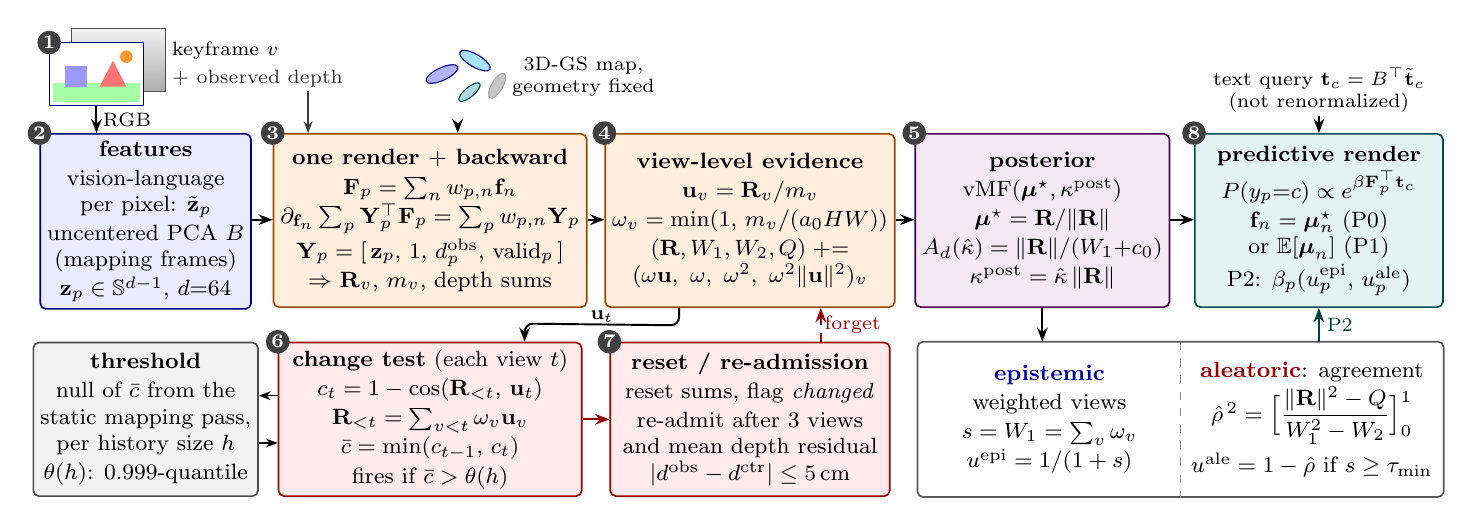
\begin{tikzpicture}[
  font=\footnotesize,
  box/.style={draw, rounded corners=2pt, line width=0.6pt, align=center, inner sep=2.5pt,
              anchor=north},
  obs/.style={box, fill=blue!8, draw=blue!50!black},
  stat/.style={box, fill=orange!13, draw=orange!60!black},
  post/.style={box, fill=violet!9, draw=violet!60!black},
  pred/.style={box, fill=teal!10, draw=teal!60!black},
  chg/.style={box, fill=red!8, draw=red!60!black},
  cal/.style={box, fill=gray!10, draw=gray!60!black},
  rowA/.style={minimum height=2.20cm},
  rowB/.style={minimum height=1.95cm},
  arr/.style={-{Stealth[length=1.8mm]}, line width=0.7pt},
  thinarr/.style={-{Stealth[length=1.5mm]}, line width=0.5pt},
  lbl/.style={font=\scriptsize, align=center, inner sep=1pt},
  num/.style={circle, fill=black!75, text=white, font=\scriptsize\bfseries, inner sep=0pt,
              minimum size=3.0mm},
]
% ---- columns: centre and width (cm); 5 columns + 4 gaps of 0.3625 cm = 17.8 cm = 7.0 in ----
\def\cA{1.325}   \def\wA{2.65}
\def\cB{4.9375}  \def\wB{3.85}
\def\cC{9.00}    \def\wC{3.55}
\def\cD{12.7125} \def\wD{3.15}
\def\cE{16.225}  \def\wE{3.15}
\def\yA{4.05}    % top of row A
\def\yB{1.40}    % top of row B
\def\yM{2.95}    % height of the row-A arrows

% ============================ row A: accumulation and read-out ============================
\node[obs, rowA, minimum width=\wA cm] (feat) at (\cA,\yA)
  {\textbf{features}\\[1pt]
   vision-language\\ per pixel: $\tilde\zv_p$\\[1pt]
   uncentered PCA $B$\\ (mapping frames)\\[1pt]
   $\zv_p\in\Sph^{d-1}$, $d{=}64$};

\node[stat, rowA, minimum width=\wB cm] (rb) at (\cB,\yA)
  {\textbf{one render $+$ backward}\\[1pt]
   $\Fv_p=\sum_n w_{p,n}\fv_n$\\[1pt]
   $\partial_{\fv_n}\sum_p\Yv_p^{\top}\Fv_p=\sum_p w_{p,n}\Yv_p$\\[1pt]
   $\Yv_p=[\,\zv_p,\,1,\,d^{\mathrm{obs}}_p,\,\text{valid}_p\,]$\\[1pt]
   $\Rightarrow$ $\R_v$,\ $m_v$,\ depth sums};

\node[stat, rowA, minimum width=\wC cm] (ev) at (\cC,\yA)
  {\textbf{view-level evidence}\\[1pt]
   $\uv_v=\R_v/m_v$\\[1pt]
   $\omega_v=\min(1,\,m_v/(a_0HW))$\\[1pt]
   $(\R,W_1,W_2,Q)\mathrel{+}=$\\
   $(\omega\uv,\ \omega,\ \omega^2,\ \omega^2\lVert\uv\rVert^2)_v$};

\node[post, rowA, minimum width=\wD cm] (post) at (\cD,\yA)
  {\textbf{posterior}\\[1pt]
   $\mathrm{vMF}(\muv^\star,\kappa^{\mathrm{post}})$\\[1pt]
   $\muv^\star=\R/\lVert\R\rVert$\\[1pt]
   $A_d(\hat\kappa)=\lVert\R\rVert/(W_1{+}c_0)$\\[1pt]
   $\kappa^{\mathrm{post}}=\hat\kappa\,\lVert\R\rVert$};

\node[pred, rowA, minimum width=\wE cm] (pred) at (\cE,\yA)
  {\textbf{predictive render}\\[1pt]
   $P(y_p{=}c)\propto e^{\beta\Fv_p^{\top}\tv_c}$\\[1pt]
   $\fv_n=\muv^\star_n$ (P0)\\ or $\mathbb{E}[\muv_n]$ (P1)\\[1pt]
   P2: $\beta_p(u^{\mathrm{epi}}_p,\,u^{\mathrm{ale}}_p)$};

% ---- row A arrows ----
\draw[arr] (feat.east |- 0,\yM) -- (rb.west |- 0,\yM);
\draw[arr] (rb.east |- 0,\yM) -- (ev.west |- 0,\yM);
\draw[arr] (ev.east |- 0,\yM) -- (post.west |- 0,\yM);
\draw[arr] (post.east |- 0,\yM) -- (pred.west |- 0,\yM);

% ============================ inputs above row A ============================
% keyframe: RGB in front, observed depth behind
\begin{scope}[shift={(0.10,4.40)}]
  \draw[draw=gray!60!black, line width=0.5pt, top color=gray!10, bottom color=gray!65]
    (0.28,0.18) rectangle ++(1.20,0.80);
  \draw[draw=blue!50!black, line width=0.5pt, fill=white] (0,0) rectangle ++(1.20,0.80);
  \fill[green!35]  (0.05,0.05) rectangle ++(1.10,0.24);
  \fill[orange!80] (0.98,0.62) circle (0.08);
  \fill[blue!40]   (0.20,0.24) rectangle ++(0.28,0.26);
  \fill[red!55]    (0.64,0.24) -- ++(0.34,0) -- ++(-0.17,0.33) -- cycle;
\end{scope}
\node[lbl, anchor=west] at (1.62,5.10) {keyframe $v$};
\node[lbl, anchor=west, gray!40!black] (dlbl) at (1.62,4.74) {+ observed depth};
\draw[arr] (0.70,4.40) -- (0.70,\yA);
\node[lbl, anchor=west] at (0.74,4.22) {RGB};
% observed depth goes straight into the backward pass
\coordinate (dIn) at ($(rb.north west)+(0.45,0)$);
\draw[thinarr, gray!45!black] (dIn |- dlbl.south) -- (dIn);

% 3D-GS map above the render box
\begin{scope}[shift={($(rb.north)+(0.15,0.30)$)}]
  \draw[fill=blue!30, draw=blue!50!black, line width=0.4pt, rotate around={25:(0,0.45)}]   (0.00,0.45) ellipse (0.22 and 0.08);
  \draw[fill=cyan!35, draw=blue!50!black, line width=0.4pt, rotate around={-30:(0.42,0.62)}] (0.42,0.62) ellipse (0.22 and 0.08);
  \draw[fill=gray!45, draw=gray!70,       line width=0.4pt, rotate around={60:(0.70,0.30)}]  (0.70,0.30) ellipse (0.18 and 0.07);
  \draw[fill=teal!30, draw=teal!60!black, line width=0.4pt, rotate around={40:(0.35,0.22)}]  (0.35,0.22) ellipse (0.17 and 0.06);
\end{scope}
\node[lbl, anchor=west] at ($(rb.north)+(1.00,0.72)$) {3D-GS map,\\ geometry fixed};
\draw[arr] ($(rb.north)+(0.35,0.12)$) -- ($(rb.north)+(0.35,0)$);

% text query above the predictive box
\node[lbl, anchor=south] (tq) at ($(pred.north)+(0,0.22)$)
  {text query $\tv_c=B^{\top}\tilde\tv_c$\\ (not renormalized)};
\draw[arr] (tq.south) -- (pred.north);

% ============================ row B: change handling and uncertainty ============================
\node[cal, rowB, minimum width=\wA cm] (cal) at (\cA,\yB)
  {\textbf{threshold}\\[1pt]
   null of $\bar c$ from the\\ static mapping pass,\\ per history size $h$\\[1pt]
   $\theta(h)$: $0.999$-quantile};

\node[chg, rowB, minimum width=\wB cm] (chg) at (\cB,\yB)
  {\textbf{change test} (each view $t$)\\[1pt]
   $c_t=1-\cos(\R_{<t},\,\uv_t)$\\[1pt]
   $\R_{<t}=\sum_{v<t}\omega_v\uv_v$\\[1pt]
   $\bar c=\min(c_{t-1},\,c_t)$\\[1pt]
   fires if $\bar c>\theta(h)$};

\node[chg, rowB, minimum width=\wC cm] (rst) at (\cC,\yB)
  {\textbf{reset / re-admission}\\[1pt]
   reset sums, flag \emph{changed}\\[1pt]
   re-admit after 3 views\\ and mean depth residual\\
   $\lvert d^{\mathrm{obs}}-d^{\mathrm{ctr}}\rvert\le 5$\,cm};

% uncertainty read-out: one box under posterior and predictive, split in two halves
\coordinate (uL) at (\cD-\wD/2,\yB);
\coordinate (uR) at (\cE+\wE/2,\yB);
\coordinate (uM) at ($(uL)!0.5!(uR)$);
\node[box, rowB, draw=none, fill=none, anchor=north, minimum width={(\cE+\wE/2-\cD+\wD/2)/2*1cm}]
  (epi) at ($(uL)!0.25!(uR)$)
  {\textbf{\color{blue!60!black}epistemic}\\[1pt]
   weighted views\\[1pt]
   $s=W_1=\sum_v\omega_v$\\[1pt]
   $u^{\mathrm{epi}}=1/(1+s)$};
\node[box, rowB, draw=none, fill=none, anchor=north, minimum width={(\cE+\wE/2-\cD+\wD/2)/2*1cm}]
  (ale) at ($(uL)!0.75!(uR)$)
  {\textbf{\color{red!60!black}aleatoric}: agreement\\[1pt]
   $\hat\rho^{\,2}=\Big[\dfrac{\lVert\R\rVert^2-Q}{W_1^2-W_2}\Big]_0^1$\\[2pt]
   $u^{\mathrm{ale}}=1-\hat\rho$ if $s\ge\tau_{\min}$};
\draw[rounded corners=2pt, line width=0.6pt, draw=black!65]
  (epi.north west) rectangle (ale.south east);
\draw[dashed, line width=0.4pt, draw=black!45] (uM) -- (uM |- ale.south);

% ---- row B arrows ----
\draw[arr] (post.south) -- (post.south |- epi.north);
\draw[arr, teal!50!black] (pred.south |- ale.north) -- (pred.south)
  node[midway, right=1.5pt, lbl] {P2};
% evidence -> change test: the current view against all earlier evidence
\draw[arr, rounded corners=3pt] ($(ev.south)+(-0.90,0)$) -- ($(ev.south)+(-0.90,-0.22)$)
  -- ($(chg.north)+(1.20,0.23)$) node[midway, above, lbl, inner sep=0.5pt] {$\uv_t$}
  -- ($(chg.north)+(1.20,0)$);
% change test <-> calibration: the mapping pass fills the null, later passes read theta
\draw[thinarr] ($(chg.west)+(0,0.30)$) -- ($(cal.east)+(0,0.30)$);    % scores c-bar (mapping)
\draw[thinarr] ($(cal.east)+(0,-0.30)$) -- ($(chg.west)+(0,-0.30)$);  % thresholds theta(h)
% change test -> reset
\draw[arr, red!60!black] (chg.east) -- (rst.west);
% reset -> sums (forget)
\draw[arr, red!60!black, dashed] ($(rst.north)+(0.90,0)$) -- ($(ev.south)+(0.90,0)$)
  node[midway, right, lbl, red!60!black] {forget};

% ---- step numbers (reading order; the caption refers to them) ----
\node[num] at (0.10,5.20) {1};
\node[num] at (feat.north west) {2};
\node[num] at (rb.north west) {3};
\node[num] at (ev.north west) {4};
\node[num] at (post.north west) {5};
\node[num] at (chg.north west) {6};
\node[num] at (rst.north west) {7};
\node[num] at (pred.north west) {8};
\end{tikzpicture}
\end{document}
